\documentclass[12pt,a4paper]{article}
\usepackage{tpl}
\dbegin[17 сентября 2019 г.]{Научный кружок}{Научный кружок}{Воропаев Алексей Сергеевич}

\hdr{Лемма Шпернера}\vskip10pt

\lemman{Шпернер} Треугольник триангулирован, и вершины раскрашены в 3 цвета так, что на ребре $n$ нет вершины цвета $n$. Тогда есть разноцветный треугольник.\label{sperner}

\proof Посмотрим на количество отрезков $1-2$. На границе треугольника их нечётно, на границе разноцветного треугольника тоже, на границе неразноцветного --- чётно. Тогда по лемме о рукопожатиях есть нечётное количество разноцветных $\triangle$, в частности, больше 0.\QEDA\\

\lemma \ref{sperner} выполнено для триангуляции многоугольников, если количество отрезков $1-2$ на границе нечётно и нет разноцветной прямой.\label{supersperner}\\

\definition{Норма} функция $f:\mathcal X\to\mathbb R_+$ со следующими свойствами:
\begin{enumerate}
	\item $f(x)=0\iff x=0$;
	\item $f(x+y)\leq f(x)+f(y)$;\label{ineq}
	\item $f(xy)=f(x)f(y)$.
\end{enumerate} Сильной нормой называется функция, где свойство \ref{ineq} заменено на неархимедово свойство --- $f(x+y)\leq\max(f(x),f(y))$.

\shdr{Свойства}
\begin{itemize}
	\item $f(1)=1$.
	\item $f(-1)=1$.
	\item $f(-a)=f(a)$.
	\item Для сильных норм $f(a)<f(b)\implies f(b-a)=f(b)$.\label{strangeness}\\
	\proof Подставим $x=b,y=-a$. Тогда $f(b-a)\leq\max(f(a),f(b))\implies f(b-a)\leq f(b)$. С другой стороны, если подставить $x=b-a,y=a$, то получится $f(b-a)\geq f(b)$ (обе подстановки в неархимедово свойство). Значит, $f(b-a)=f(b)$.\QEDA
\end{itemize}

\definition{$p$-адическая норма $N_2$} норма, определяемая для рациональных $x$ как $2^{-n}$, где $n$ --- степень вхождения $2$ в $x$ ($N_2(0)=0$ по определению; заметим, что это сильная норма над $\mathbb Q$).\\

\theoremn{Лэнг} Неархимедова норма над $\mathbb Q$ продолжается на $\mathbb R$.\\

\theorem Квадрат нельзя разрезать на нечётное количество равновеликих треугольников.

\proof Пусть $1=n\cdot S$, где $n$ --- количество треугольников, $S$ --- площадь. Докажем, что у $S$ чётный знаменатель. Заметим, что $N_2(1)=N_2(n)N_2(S)$, т.е. $N_2(S)\geq1$, причём равно, только если $n$ нечётно. 

Покрасим все точки квадрата $1\times 1$ в три цвета так. Красим точку $(x,y)$ в красный, если $N_2(x)<1,N_2(y)<1$, в синий, если $N_2(x)\geq1, N_2(x)\geq N_2(y)$, в зелёный, если $N_2(y)\geq1, N_2(y)>N_2(x)$.

\lemma Пусть точка $K$ красная. Тогда цвета точек $P$ и $P-K$ совпадают.

\proof Рассмотрим 2 случая:
\begin{enumerate}
	\item $P$ красная. Тогда по неархимедовости $N_2(x_P-x_A)$ меньше единицы, аналогично для $y$.\QEDA
	\item $P$ не красная. Пусть она синяя. Тогда $x$ всё ещё больше единицы, а $y$ либо не изменился, либо остался меньше единицы.\QEDA
\end{enumerate}

\lemma Условие \ref{supersperner} выполнено.

\proof Пусть есть точки $R,G,B$ на одной прямой. Тогда точки $0,G-R,B-R$ тоже на одной прямой и тех же цветов. С другой стороны, если 2 точки и 0 на одной прямой, они не могут быть одна синей, а другая зелёной, т.к. тогда в одной $\frac{x}{y}$ больше единицы, а в другой меньше. Значит, трёхцветных прямых нет. Теперь посмотрим, например, на красно-синие отрезки. На участке $R-U-U$ их нечётно, а на сторонах $U-G$ и $G-R$ их нет.\QEDA\\

\textbf{Завершение доказательства.} Применением \ref{supersperner} мы нашли разноцветный треугольник. Его можно сдвинуть в 0, пусть его
остальные вершины --- $(x_1,y_1)$ и $(x_2,y_2)$. Тогда его площадь --- $\pm\frac{x_1y_2-x_2y_1}2$. Посчитаем от этой площади $N_2$. Это $2N_2(x_1y_2-x_2y_1)$. Заметим, что $N_2(x_1)\geq N_2(y_2)$ и $N_2(y_2)>N_2(x_1)$ из-за цвета точек, тогда $2N_2(x_1y_2-x_2y_1)=2N_2(x_1)N_2(y_2)\geq2$.\QEDA\\

\newpage
\hdr{Стрельба по черепашкам}\vskip10pt


Возьмём какой-нибудь многочлен (для примера, $P(x)=x^3+4x^2+5x+2$) и пустим черепашку:

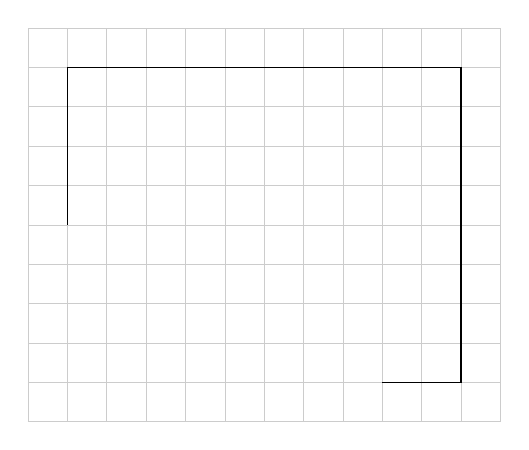
\begin{tikzpicture}
	\draw[step=0.5,very thin,black!20] (-4.5,-0.5) grid (1.5,4.5);
	\path[draw] (0,0)--(1,0)--(1,4)--(-4,4)--(-4,2);
\end{tikzpicture}

Будем пускать лазер, который отражается от стенок под углом $90^\circ$ (при этом мы имеем в виду не луч, а прямую, и стенки --- тоже прямые):

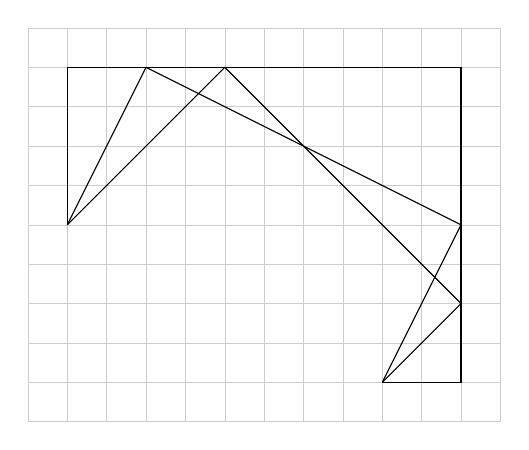
\begin{tikzpicture}
	\draw[step=0.5,very thin,black!20] (-4.5,-0.5) grid (1.5,4.5);
	\path[draw] (0,0)--(1,0)--(1,4)--(-4,4)--(-4,2);
	\path[draw] (0,0)--(1,1)--(-2,4)--(-4,2);
	\path[draw] (0,0)--(1,2)--(-3,4)--(-4,2);
\end{tikzpicture}

\lemma $x$ --- корень $P(x)\ \iff$ лазер под углом наклона $arctg(-x)$ попадает в голову.

\proof Сделаем один шаг лазера. Тогда получится $P(x)-a_nx^{n-1}(x+\alpha)$, где $\alpha$ --- тангенс угла наклона лазера. После $n$ шагов получим $P(x)-Q(x)(x+\alpha)$, т.е. это деление с остатком. \QEDA\\

\textbf{Следствие.} Если у нечётных коэффициентов поменять знаки, то у корня поменяется знак.

\textbf{Следствие.} Если коэффициенты поменять местами, то корень поменяется на обратный.\\

\lemma Пусть $\alpha$ --- корень $P$. Тогда если взять в качестве новых коэффициентов длины отрезков лазера, получится новый многочлен, у которого корни --- все корни $P$, кроме $\alpha$.

\proof Следует из теоремы Безу. \QEDA\\

Пусть $P(x)$ квадратный. Тогда можно заметить, что корни --- пересечение окружности с диаметром $A_0A_3$ с прямой $A_1A_2$. Тогда для них $y=0$ и $(x-\frac{b}{2})^2+(y-\frac{a+c}{2})^2=\frac{b^2+(c-a)^2}{4}$, т.е. мы снова вывели формулу через дискриминант. Также можно найти этот корень циркулем.

\begin{tikzpicture}
	\draw[step=0.5,very thin,black!20] (-3.5,-0.5) grid (1.5,4.5);
	\path[draw] (0,0)--(1,0)--(1,4)--(-2,4);
	\path[draw] (0,0)--(1,1)--(-2,4);
	\node[draw] at(-1,2) [circle through={(1,1)}] {};
	\path[draw] (0,0)--(1,3)--(-2,4);
\end{tikzpicture}

\newpage
\shdr{Оригами}\vskip8pt
Отразим точку $A_0$ относительно $A_1$. Получим точку, которая лежит на какой-то фиксированной прямой, и складка листа проходит через $A_2$. То есть мы свели построение окружности к 5 правилу Фудзиты. Аналогично можно свести решение кубического уравнения к 6 правилу Фудзиты.

\begin{tikzpicture}
	\draw[step=0.5,very thin,black!20] (-3.5,-0.5) grid (2.5,4.5);
	\path[draw] (0,0)--(1,0)--(1,4)--(-2,4);
	\path[draw,dashed] (1,1)--(-2,4);
	\node[draw] at(-1,2) [circle through={(1,1)}] {};
	\path[draw] (0,0)--(2,2)--(-2,4)--(0,0);
\end{tikzpicture}

Возьмём любую точку $P$ внутри черепашки и построим ГМТ $X$ таких: отображаем оригами $l$ на $P$, затем проводим перпендикуляр в $P$ и пересекаем с биссектрисой. Тогда это ГМТ --- парабола с фокусом $P$ и директрисой $l$, а биссектриса --- касательная к параболе.

Теперь мы решаем кубическое уравнение и отображаем две прямые на две точки. На самом деле, это построение общей касательной к двум параболам.

\hdr{Комплексный случай}
Пусть $P(x)=x^3+4x^2+9x+10$. Тогда у него два комплексных корня. Тогда $A_i$ --- $\triangle$.

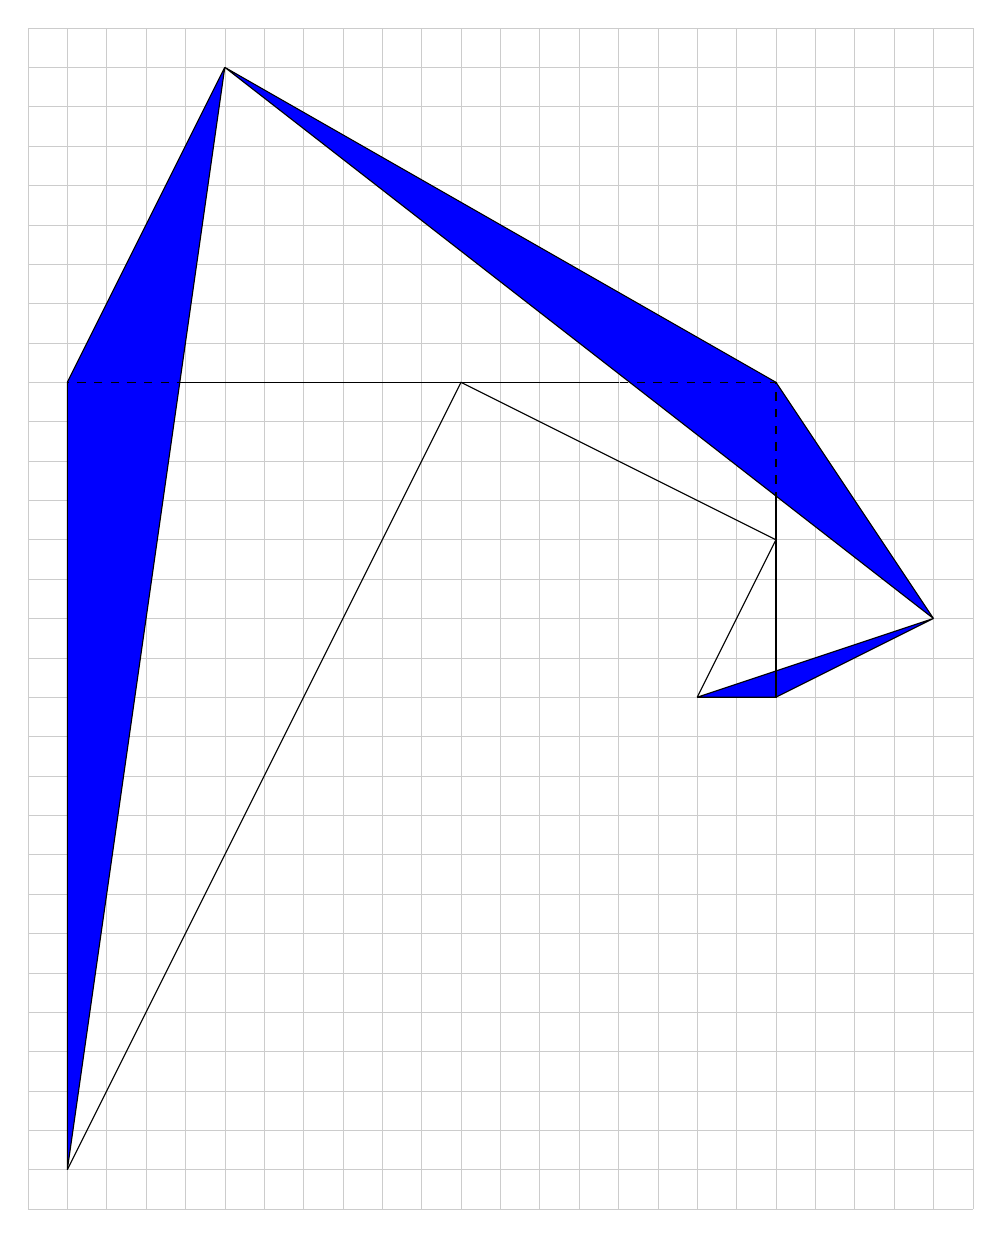
\begin{tikzpicture}
	\draw[step=0.5,very thin,black!20] (-8.5,-6.5) grid (3.5,8.5);
	\draw[fill=blue] (0,0)--(3,1)--(1,0)--(0,0);
	\draw[fill=blue] (3,1)--(-6,8)--(1,4)--(3,1);
	\draw[fill=blue] (-6,8)--(-8,4)--(-8,-6)--(-6,8);
	\path[draw] (0,0)--(1,0)--(1,2.5);
	\path[draw,dashed] (1,2.5)--(1,4)--(-1,4);
	\path[draw] (-1,4)--(-6.5,4);
	\path[draw,dashed] (-6.5,4)--(-8,4);
	\path[draw] (0,0)--(1,2)--(-3,4)--(-8,-6);
\end{tikzpicture}
\end{document}
